\documentclass[../thesis.tex]{subfiles}
\graphicspath{{../gfx/}{gfx/}}
\begin{document}

\pagestyle{plain}

\chapter{Projekt systemu komputerowego}

Rozdział ten skupia się nad projektem systemu komputerowego umożliwiającego porównywanie jakości klasyfikacji dla różnych grup algorytmów. Aplikacja jest podzielona na oddzielne, współpracujące ze sobą, elementy. Zaproponowany przeze mnie system komputerowy składa się z gotowych komponentów, o którym mowa w części \ref{proj:arch}, oraz z fragmentów, które należy, chociaż w pewnej części, zaimplementować samodzielnie. W skład tych części wchodzi przede wszystkim biblioteka obliczeniowa \emph{mltool}, program wykonujący obliczenia, program nadzorujący przeprowadzanie obliczeń oraz programy prezentujące ostateczne wyniki.

\section{Architektura systemu}
\label{proj:arch}

Dzięki rozdzieleniu całości na powiązane, lecz odrębne, moduły, prace nad wybranym fragmentem systemu można prowadzić w oderwaniu od reszty. Dodatkowo, luźno powiązana architektura umożliwia testowanie każdego podsystemu oddzielnie. Upraszcza to znacząco testowanie całej aplikacji.

\subsection{Przegląd rozwiązań}

System komputerowy powinien być w stanie prowadzić obliczenia na wielu maszynach w sposób równoległy (patrz: \ref{req:research_scheme}). Jedną z metod rozwiązania takiego problemu mogłoby być użycie platformy \emph{Apache Hadoop}. System ten jest otwartą implementacją paradygmatu \emph{MapReduce} firmy Google. Platforma Hadoop umożliwia równoległe przetwarzanie danych tekstowych na wielu maszynach. System ten zapewnia ciągłą pracę w momencie awarii niektórych maszyn wykonujących obliczenia. Z punktu widzenia pracy dyplomowej, system Apache Hadoop posiada jednak pewne wady. 

Po pierwsze, jest on zaprojektowany do równoległego przetwarzania danych tekstowych (np. zliczania częstości występowania słów w tekście). Z drugiej strony, obliczenia w projektowanym systemie polegać będą na równoległym obliczaniu miar jakości klasyfikacji algorytmów. Aby pogodzić wymagania systemu z funkcjonalnością platformy Hadoop należałoby przygotować oprogramowanie reprezentujące oceniane algorytmy w postaci tekstowej zrozumiałej przez system Hadoop. 

Po drugie, platforma Hadoop jest wysoko rozwiniętym i skomplikowanym systemem. Uruchomienie klastra obliczeniowego wiązałoby się z długim czasem poświęconym na dostrajanie konfiguracji systemu.

Alternatywnym rozwiązaniem jest użycie rozproszonego systemu kolejkowego tj. \emph{Apache ActiveMQ}, \emph{RabbitMQ} lub \emph{ZeroMQ}. Podstawowym zadaniem systemów kolejkowych jest kolejkowanie zleceń wykonania pewnych czynności (np. obliczeń) i późniejsze rozsyłanie ich pomiędzy procesy realizujące te zlecenia. Systemy kolejkowe pozwalają na elastyczne definiowanie przepływu danych pomiędzy różnymi kolejkami. 

W odróżnieniu od platformy Hadoop, procesy wykonujące zlecenia odbierają je w jako komunikaty, bardzo często dowolnej postaci. Systemy kolejkowe są również z reguły proste do opanowania i nie wymagają skomplikowanej konfiguracji od użytkownika. Wadą systemów kolejkowych jest brak odporności na awarie procesów-odbiorców oraz maszyn, na których procesy te są uruchomione. Mając na uwadze, że czas obliczeń w projektowanym systemie nie powinien przekraczać kilku dni, prawdopodobieństwo awarii i ryzyko z nim związane jest pomijalne. W związku z tym, dwie wymienione zalety zadecydowały o wyborze architektury opartej na systemie kolejkowym.

\subsection{Opis architektury}

System komputerowy składa się z \emph{procesów-robotników} wykonujących ciężkie obliczenia (związane z oceną klasyfikacji) oraz pojedynczego \emph{procesu-nadzorcy} rozdzielającego zadania do wykonania. Dodatkowym zadaniem nadzorcy jest odbieranie cząstkowych wyników od każdego robotnika i umieszczanie ich w bazie danych. Komunikacja pomiędzy nadzorcą a robotnikami jest zapewniona poprzez zastosowanie systemu kolejkowego RabbitMQ. System ten został wybrany ze względu na cenę (darmowy), prostotę instalacji, wysoką wydajność oraz bardzo dobre wsparcie w wielu językach programowania (np. w języku Python).

Dane przechowywane są w wolno dostępnej bazie \emph{PostgreSQL}. Wybierając bazę danych kierowałem się przede wszystkim ceną (baza darmowa), łatwością instalacji i konfiguracji oraz wydajnością. Na wybór bazy miały wpływ również moja znajomość języka SQL oraz obecność wielu narzędzi mapowania obiektowo-relacyjnego, uproszczających pracę z danymi. 

Proces nadzorujący oraz procesy wykonujące obliczenia używają wspólnej biblioteki obliczeniowej \emph{mltool}. 

Programy służące do prezentacji wyników obliczeń dla każdej grupy algorytmów oraz do policzenia rankingu grup pobierają dane z bazy PostgreSQL oraz również używają biblioteki \emph{mltool}.

Poglądowy schemat architektury systemu komputerowego umieszczony został na rysunku \ref{proj:arch_diagram}.

\begin{figure}[h]
\centering
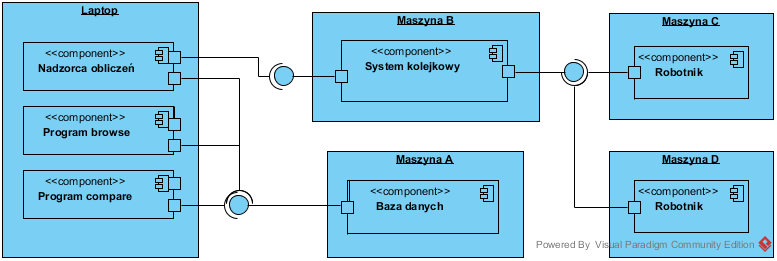
\includegraphics[width=\textwidth]{arch.png}
\caption{Schemat architektury systemu komputerowego}
\label{proj:arch_diagram}
\end{figure}

\section{Biblioteka obliczeniowa mltool}

\subsection{Struktura biblioteki}
\label{proj:sec_structure}

Biblioteka obliczeniowa składa się z czterech części. Pierwszą z nich jest zbiór klas odpowiedzialnych za odczyt i dostęp do danych biomedycznych. W skład drugiej części biblioteki wchodzą klasy pozwalające na manipulowanie danymi (np. na skalowanie atrybutów) oraz na ich klasyfikację. Kolejną częścią biblioteki są klasy związane z przetwarzaniem wstępnym i klasyfikacją danych w sposób zdefiniowany przez użytkownika. Stanowią one sparametryzowany opis operacji, jakie powinny być wykonane przez proces liczący (robotnika). Ostatnim fragmentem biblioteki obliczeniowej są klasy związane z generowaniem algorytmów przetwarzania i klasyfikacji odpowiadających opisowi danej grupy algorytmów.

\subsection{Odczyt danych}

W części tej znajdują się opisy klas odpowiedzialnych za odczyt i właściwą reprezentację danych.

\subsubsection{Interfejs TabularFile}

Zadaniem interfejsu \emph{TabularFile} jest zapewnienie warstwy abstrakcji pomiędzy odczytem danych z pliku, a interpretacją danych w nim zgromadzonych. Jeżeli projekt będzie rozwijany w przyszłości, może okazać się, że pojawi się potrzeba odczytu plików różnych rodzajów (np. CSV lub formaty binarne). Obecność ujednoliconego interfejsu uprości w takim przypadku rozwój systemu.

Interfejs posiada tylko dwie metody: \emph{columns()} oraz \emph{rows()}. Pierwsza z nich zwraca tablicę nazw kolumn w pliku. Druga zwraca tekstową tablicę dwuwymiarową odpowiadającą kolejnym wierszom danych w pliku.

\subsubsection{Klasa XlsFile}

W tym momencie przewidywana jest tylko jedna implementacja interfejsu \emph{TabularFile} - klasa \emph{XlsFile}. Klasa ta pozwala na odczyt danych zgromadzonych w postaci tabeli z pliku MS Excel. Diagramy interfejsu \emph{TabularFile} oraz klasy \emph{XlsFile} prezentuje rysunek \ref{proj:diagram_xls_file}.

\begin{figure}[h]
\centering
\begin{tikzpicture} 
\umlclass{XlsFile}{
}{
  \umlstatic{+ load(filepath: String): XlsFile}\\
  + XlsFile(filepath: String)\\
  + columns(): Array[String]\\
  + read()\\
  + rows(): Array[Array[String]]\\
}
\umlclass[x=8,y=0,type=interface]{TabularFile}{
}{
  + columns(): Array[String]\\
  + rows(): Array[Array[String]]\\
}
\umlimpl{XlsFile}{TabularFile}
\end{tikzpicture}
\caption{Diagram UML interfejsu \emph{TabularFile} i klasy \emph{XlsFile}}
\label{proj:diagram_xls_file}
\end{figure}

Konstruktor klasy \emph{XlsFile} przyjmuje ścieżkę do pliku z danymi. Metoda \emph{read()} ładuje zawartość pliku do obiektu klasy. Statyczna metoda \emph{load()} zwraca załadowany obiekt klasy \emph{XlsFile}. Jej jedynym argumentem jest ścieżka do pliku. Metody \emph{columns()} oraz \emph{rows()} to implementacje metod interfejsu \emph{TabularFile}.

\subsubsection{Klasa Sample}

Klasa \emph{Sample} stanowi reprezentację próbki danych zawartych w pliku dostarczonym przez użytkownika. Klasa ta zawiera pola odpowiadające cechom próbki (liczba wierszy, liczba i nazwy atrybutów) jak również udostępnia metody manipulujące danymi. Instancje obiektów klasy \emph{Sample} przechowują wyłącznie atrybuty o ustalonych wartościach numerycznych. Wartości brakujące reprezentowane są prze numeryczną wartość \emph{NaN} (ang.\emph{ Not A Number}). Pola i metody klasy prezentuje diagram \ref{proj:diagram_sample}.

\begin{figure}[h]
\centering
\begin{tikzpicture} 
\umlclass{Sample}{
  + attributes: Array[Array[Float]]\\
  + categories: Array[Float]\\
  + columns: Array[String]\\
  + ncols: Int\\
  + nrows: Int\\
}{
  \umlstatic{+ fromFile(file: TabluarFile, rowIndices: Array[Int]) : Sample}\\
  + get\_normalizer(target: Tuple[Float, Float])\\
  + impute(model: Imputer)\\
  + merge(clusterer: Clusterer)\\
  + normalize(normalizer: Normalizer, columns: Array[String])\\
  + remove\_columns(columns: Array[String])\\
}
\end{tikzpicture}
\caption{Diagram UML klasy \emph{Sample}}
\label{proj:diagram_sample}
\end{figure}

Pole \emph{attributes} jest tablicą dwuwymiarową przechowującą informacje o wartościach numerycznych poszczególnych atrybutów. Pole \emph{categories} to tablica wartości numerycznych odpowiadających kategoriom kolejnych przykładów (0 - stan chorobowy, 1 - brak stanu chorobowego). Pole \emph{columns} to tablica nazw kolejnych atrybutów. Pola \emph{ncols} i \emph{nrows} przechowują informacje o liczbie kolumn i liczbie przykładów w próbce danych.

Statyczna funkcja \emph{fromFile()} służy do utworzenia obiektu klasy \emph{Sample} na podstawie istniejącego obiektu klasy $t_f$ implementującej interfejs \emph{TabularFile}. Funkcja ta jako argumenty przyjmuje obiekt $t_f$ oraz, opcjonalnie, tablicę indeksów wierszy, które należy wybrać z obiektu $t_f$.

Metoda \emph{get\_normalizer()} zwraca obiekt klasy Normalizer, stanowiący model skalowania atrybutów w zbiorze danych (patrz: \ref{proj:models}). 

Zadaniem metody \emph{impute()} jest imputacja brakujących wartości atrybutów w próbie danych zawartej w obiekcie klasy \emph{Sample}. Metoda ta przyjmuje pojedynczy argument - obiekt klasy \emph{Imputer}, będący model imputacji danych.

Celem metody \emph{merge()} jest zgrupowanie wybranych atrybutów ze zbioru danych wg reguł ustalonych w obiekcie \emph{Clusterer} (atrybuty do pogrupowania, algorytmy grupowania oraz parametry tych algorytmów). Parametrem metody jest obiekt klasy \emph{Clusterer}.

Metoda \emph{normalize()} ma za zadanie przeskalować wybrane atrybuty ze zbioru danych. Parametrami metody są obiekt klasy \emph{Normalizer} oraz tablica nazw atrybutów, które mają zostać przeskalowane.

Ostatnią metodą klasy \emph{Sample} jest \emph{remove\_columns()}. Zgodnie z tym, co wskazuje nazwa, metoda usuwa ze zbioru danych wybrane atrybuty. Argumentem metody jest tablica nazw atrybutów do usunięcia.

\subsection{Modele przetwarzania i klasyfikacji}
\label{proj:models}

Efektem działania algorytmu przetwarzania wstępnego i klasyfikacji jest wytworzenie modelu, który w pewien sposób opisuje wiedzę zawartą w danych. Model ten wytwarzany jest przy użyciu danych trenujących i wykorzystywany jest do predykcji kategorii, nieznanych wcześniej, danych testowych. 

Model powinien uwzględniać wszystkie etapy algorytmu, a fazy przetwarzania i klasyfikacji. Model przetwarzania musi przechowywać informacje o cechach danych istotnych z punktu widzenia transformacji danych. Model taki powinien opisywać cechy szczególne danych pod kątem kolejnych operacji, czyli imputacji brakujących wartości, usuwania atrybutów, skalowania atrybutów i ich późniejszego grupowania.

Model klasyfikacji powinien tworzyć reprezentację wiedzy zawartej w danych w taki sposób, aby możliwe było wykorzystanie jej do późniejszej predykcji nowych danych.

Z punktu widzenia projektu aplikacji, modele powinny udostępniać zbliżony interfejs programistyczny. Interfejs ten w każdym przypadku powinien zawierać przynajmniej jedną metodę o nazwie \emph{fit}. Metoda ta jest odpowiedzialna za wygenerowanie modelu z dostępnych danych. Dodatkowo, modele przetwarzania muszą posiadać metodę \emph{transform} służącą do transformacji pojedynczego wiersza danych zgodnie z uzyskanym modelem. Modele klasyfikacji powinny posiadać metodę \emph{predict}, której użycie zwracałoby przewidywaną kategorię przykładu.

\subsubsection{Klasa Imputer}

Klasa \emph{Imputer} służy do imputacji brakujących danych atrybutów. Konstruktor klasy może przyjmować pojedynczą wartość oznaczającą metodę imputacji. Poprawnymi wartościami parametru są \emph{mean} oraz \emph{median}. Metoda \emph{fit} przyjmuje również tylko jeden parametr - dwuwymiarową tablicę zawierającą wartości atrybutów (w tym braki oznaczone jako \emph{NaN}). Metoda transform pobiera jeden argument będący dwuwymiarową tablicę wartości atrybutów. Po wywołaniu metody wartości \emph{NaN} występujące w tablicy zostają zastąpione przez średnią lub medianę odpowiedniego atrybutu. 

Rysunek \ref{proj:diagram_imputer} ilustruje wygląd klasy \emph{Imputer}.

\begin{figure}[h]
\centering
\begin{tikzpicture} 
\umlclass{Imputer}{
}{
  + fit(attributes: Array[Array[Float]])\\
  + transform(attributes: Array[Array[Float]])\\
}
\end{tikzpicture}
\caption{Diagram UML klasy \emph{Imputer}}
\label{proj:diagram_imputer}
\end{figure}

\subsubsection{Klasa Normalizer}

Zadaniem klasy \emph{Normalizer} jest przechowywanie informacji o numerycznym zakresie wartości poszczególnych atrybutów. Po wygenerowaniu modelu, klasa \emph{Normalizer} może być użyta do przeskalowania wartości atrybutu do ustalonego zakresu. 

Parametrem konstruktora klasy jest para liczb odpowiadająca zakresowi liczbowemu $z$, do którego powinny być przeskalowane napływające dane.

Klasa posiada dwie metody: \emph{fit} oraz \emph{transform}. Metoda \emph{fit} posiada jeden parametr - obiekt klasy \emph{Sample}. Efektem wywołania metody \emph{fit} jest wytworzenie modelu zakresu atrybutów danych. 

Zadaniem metody \emph{transform} jest przeskalowanie danych wejściowych do wybranego zakresu liczbowego $z$. Metoda posiada dwa argumenty. Pierwszy z nich to obiekt klasy \emph{Sample}, którego atrybuty mają zostać przeskalowane. Drugi argument to tablica nazw atrybutów, które mają być poddane skalowaniu.

Klasa \emph{Normalizer} jest przedstawiona na rysunku \ref{proj:diagram_normalizer}.

\begin{figure}[h]
\centering
\begin{tikzpicture} 
\umlclass{Normalizer}{
}{
  + Normalizer(start: Float, end: Float)\\
  + fit(sample: Sample)\\
  + transform(sample: Sample, columns: Array[String])\\
}
\end{tikzpicture}
\caption{Diagram UML klasy \emph{Normalizer}}
\label{proj:diagram_normalizer}
\end{figure}

\subsubsection{Klasa Clusterer}

Celem klasy \emph{Clusterer} jest wytworzenie modelu grupowania danych, zgodnego z ustawieniami użytkownika, oraz późniejsze grupowanie nowych danych przy użyciu tego modelu. 

Konstruktor klasy \emph{Clusterer} pobiera jeden argument będący tablicą obiektów klasy \emph{GroupingDescriptor}. Każdy obiekt klasy posiada informację o szczegółach grupowania podzbioru atrybutów. Szczegółowy opis klasy \emph{GroupingDescriptor} znajduje się w części \ref{proj:descriptors}.

Klasa posiada dwie metody: \emph{fit} oraz \emph{transform}. Metoda fit posiada jeden argument - obiekt klasy \emph{Sample}. Po wywołaniu metody fit obiekt klasy \emph{Clusterer} tworzy wewnętrzny model wiedzy dotyczącej grupowania atrybutów w zbiorze danych.

Metoda transform posiada również tylko jeden parametr, będący ponownie obiektem klasy \emph{Sample}. Efektem wywołania metody \emph{transform} jest pogrupowanie atrybutów w zbiorze danych zgodnie z modelem wytworzonym metodą \emph{fit}.

Na rysunku \ref{proj:diagram_clusterer} przedstawiono metody klasy \emph{Clusterer}.

\begin{figure}[h]
\centering
\begin{tikzpicture} 
\umlclass{Clusterer}{
}{
  + Clusterer(descriptors: Array[GroupingDescriptor])\\
  + fit(sample: Sample)\\
  + transform(sample: Sample)\\
}
\end{tikzpicture}
\caption{Diagram UML klasy \emph{Clusterer}}
\label{proj:diagram_clusterer}
\end{figure}

\subsubsection{Usuwanie atrybutów}

W przypadku usuwania atrybutów ze zbioru danych nie jest potrzeby żaden specjalny model wiedzy. Aby w jednakowy sposób pozbyć się atrybutów w zbiorze trenującym i testowym wystarczy utworzyć tablicę nazw atrybutów, które należy usunąć.

\subsubsection{Interfejs Classifier}

Interfejs \emph{Classifier} zapewnia możliwość nauki modelu klasyfikacji oraz predykcji kategorii nowych przykładów. Interfejs ma dwie metody: \emph{fit()} i \emph{predict()}.

\begin{figure}[h]
\centering
\begin{tikzpicture} 
\umlclass[type=interface]{Classifier}{
}{
  \umlvirt{+ fit(attributes: Array[Array[Float]])}\\
  \umlvirt{+ predict(data: Array[Float]): Int}\\
}
\umlemptyclass[x=-5,y=-3]{NaiveBayesClassifier}
\umlemptyclass[x=-3,y=-5]{DecisionTreeClassifier}
\umlemptyclass[x=+3,y=-5]{SVMClassifier}
\umlemptyclass[x=+5,y=-3]{RandomForestClassifier}
\umlimpl[geometry=--]{NaiveBayesClassifier}{Classifier}
\umlimpl[geometry=--]{DecisionTreeClassifier}{Classifier}
\umlimpl[geometry=--]{SVMClassifier}{Classifier}
\umlimpl[geometry=--]{RandomForestClassifier}{Classifier}
\end{tikzpicture}
\caption{Diagram UML interfejsu \emph{Classifier}}
\label{proj:diagram_classifier}
\end{figure}

Metoda \emph{fit()} służy do nauki modelu danych. Metoda ta przyjmuje pojedynczy parametr będący tablicą dwuwymiarową zawierającą wartości atrybutów zbioru danych. Po wywołaniu tej metody obiekt implementujący interfejs \emph{Classifier} wytwarza swój własny model klasyfikacji.

Zadaniem metody \emph{predict()} jest predykcja kategorii przykładu ze zbioru danych. Metoda przyjmuje tablicę wartości odpowiadającą pojedynczemu przykładowi ze zbioru danych. Wynikiem wywołania metody jest wartość predykcji - przewidywana kategoria przykładu.

Interfejs \emph{Classifier} jest zaimplementowany przez cztery klasy: \emph{NaiveBayesClassifier}, \emph{DecisionTreeClassifier}, \emph{SVMClassifier} oraz \emph{RandomForestClassifier}. Odpowiadają one algorytmom klasyfikacji naiwny klasyfikator bayessowski, drzewo decyzyjne, maszyna wektorów nośnych i las losowy. Całość przedstawia rysunek \ref{proj:diagram_classifier}.

\subsection{Deskryptory operacji}
\label{proj:descriptors}

Projektując bibliotekę postanowiłem oddzielić kod związany z wyborem parametrów przetwarzania od kodu wykonującego to przetwarzanie. W tym celu zaprojektowałem specjalne klasy, tzw. \emph{deskryptory}. Klasy te czerpią ze wzorca projektowego \emph{Polecenie}~\cite{gang_of_four}, stanowiąc opisy operacji, które mają zostać wykonane. Każdy z deskryptorów dotyczy szczególnej części przetwarzania i posiada metody wykonujące daną operację oraz metody sprawdzające poprawność opisu operacji.

Użycie deskryptorów posiada wiele zalet. Po pierwsze, logika związana z definiowaniem kolejnych kroków algorytmu jest odseparowana do właściwego algorytmu. Efektem tego jest prostszy i czytelniejszy kod. Po drugie, każdy deskryptor posiada metody umożliwiające sprawdzenie, czy wprowadzony opis operacji jest poprawny. Pomaga to w zarządzaniu kodem związanym z nieprawidłowymi ustawieniami wprowadzonymi przez użytkownika. Kolejną zaletą jest ograniczenie duplikacji kodu. Zarówno funkcjonalność związana z przetwarzaniem danych jak i ta polegająca na przeszukiwaniu mogą wykorzystywać klasy deskryptorów. Dodatkowym atutem podziału kodu na deskryptory jest uproszczenie testów jednostkowych. Testy projektowane będą pod określony deskryptor, dzięki czemu ich kod będzie czytelniejszy i prostszy w utrzymaniu.

Warto również spojrzeć na kwestię rozproszonego wykonywania obliczeń. Użycie klas, jakimi są deskryptory, umożliwi rozdzielenie kodu odpowiedzialnego za wytwarzanie deskryptorów od kodu przetwarzającego dane zgodnie z opisem zawartym w deskryptorach. Rozdzielenie tych obowiązków posiada bardzo dużą zaletę. Na komputerach wyposażonych w przynajmniej dwa rdzenie procesora aplikacja będzie mogła w prosty sposób przetwarzać dane równolegle. Możliwość ta wynika z faktu, że wygenerowanie pojedynczego deskryptora zajmować będzie znacznie mniej czasu, niż przetworzenie danych związanych z nim. Wątek (lub proces) będzie ,,rozdawał'' opisy operacji innym wątkom (lub procesom) i co jakiś czas odbierał rezultaty obliczeń. Rozwiązanie to pozwoli na skrócenie czasu przeszukiwania.

\subsubsection{Klasa PreprocessingDescriptor}

W mojej pracy planuję zaimplementować trzy rodzaje deskryptorów. Pierwszym z nich jest klasa \emph{PreprocessingDescriptor} związana ze wstępnym przetwarzaniem danych. Instancje obiektu klasy \emph{PreprocessingDescriptor} posiadają pola zawierające informacje o metodzie radzenia sobie z brakującymi danymi, atrybutach poddawanych skalowaniu itd. Diagram \ref{proj:diagram_preprocessing_descriptor} przedstawia pola i metody klasy.

\begin{figure}[h]
\centering
\begin{tikzpicture} 
\umlclass{PreprocessingDescriptor}{
  + imputeMethod: String\\
  + removeCols: Array[String]\\
  + scaleCols: Array[String]\\
  + groupDescr: Array[GroupingDescriptor]\\
}{
  + PreprocessingDescriptor(imputeMethod: String, removeCols: Array[String],\\ scaleCols: Array[String], groupDescr: Array[GroupingDescriptor])\\
  + cluster(sample: Sample)\\
  + impute(sample: Sample)\\
  + validate()\\
}
\end{tikzpicture}
\caption{Diagram UML klasy \emph{PreprocessingDescriptor}}
\label{proj:diagram_preprocessing_descriptor}
\end{figure}

Klasa \emph{PreprocessingDescriptor} posiada cztery pola. Pole \emph{imputeMethod} oznacza rodzaj metody imputacji brakujących wartości atrybutów w zbiorze danych. Pole \emph{removeCols} to tablica nazw atrybutów, które powinny zostać usunięte ze zbioru danych w trakcie przebiegu algorytmu. Pole \emph{scaleCols} jest tablicą nazw atrybutów, które powinny zostać przeskalowane do przedziału [-1, 1]. Ostatnie pole, \emph{groupDescr}, to tablica obiektów klasy \emph{GroupingDescriptor}, opisujących grupowanie atrybutów w zbiorze.

Konstruktor klasy przyjmuje cztery parametry odpowiadające wartościom pól klasy.

W klasie powinny zostać zaimplementowane dwie metody wytwórcze: \emph{cluster()} oraz \emph{impute()}. Pierwsza z metod przyjmuje jako parametr obiekt klasy \emph{Sample} $s_1$. Wynikiem metody jest obiekt klasy \emph{Clusterer} z wewnętrznym modelem wytworzonym na obiekcie $s_1$. 

Na podobnej zasadzie działa metoda o nazwie \emph{impute}. Metoda przyjmuje pojedynczy argument - obiekt klasy \emph{Sample} $s_2$ - i zwraca obiekt klasy \emph{Imputer} nauczony na obiekcie $s_2$.

Dodatkowo, klasa \emph{PreprocessingDescriptor} posiada metodę \emph{validate()}. Metoda ta ma za zadanie sprawdzić, czy pola klasy mają poprawne wartości. Jeżeli wartości są niepoprawne, metoda rzuca wyjątek typu \emph{DescriptorException}.

\subsubsection{Klasa GroupingDescriptor}

Następnym deskryptorem jest klasa \emph{GroupingDescriptor}. Przechowuje ona informacje o grupowaniu atrybutów danych z wykorzystaniem pojedynczego, określonego algorytmu grupowania (np. K-Średnich). Poza metodą sprawdzającą, klasa \emph{GroupingDescriptor} oferuje również metodę wytwórczą createAlgorithm. Pola i metody klasy przedstawia diagram \ref{proj:diagram_grouping_descriptor}.

\begin{figure}[h]
\centering
\begin{tikzpicture} 
\umlclass{GroupingDescriptor}{
  + columns: Array[String]\\
  + groupingArgs: Array[String]\\
  + groupingMethod: String\\
}{
  + GroupingDescriptor(columns: Array[String], groupingArgs: Array[String],\\ groupingMethod: String)\\
  + createAlgorithm(): GroupingAlgorithm\\
  + validate()\\
}
\end{tikzpicture}
\caption{Diagram UML klasy \emph{GroupingDescriptor}}
\label{proj:diagram_grouping_descriptor}
\end{figure}

Konstruktor klasy \emph{GroupingDescriptor} posiada trzy parametry. Pierwszy z nich to tablica nazw atrybutów, które mają być poddane grupowaniu. Drugi parametr to tablica wartości, które odpowiadają parametrom wybranego algorytmu grupowania. W zależności od wyboru metody grupowania, tablica ta może mieć różną długość. Ostatnim parametrem konstruktora jest nazwa metody grupowania, np. \emph{k-means.}

Pola klasy w dokładny sposób odpowiadają parametrom konstruktora klasy.

Klasa posiada metodę wytwórczą \emph{createAlgorithm()}. Zadaniem tej metody jest stworzenie obiektu pozwalającego na grupowanie zgodnie z ustaloną metodą i jej parametrami. Metoda zwraca obiekt implementujący interfejs \emph{GroupingAlgorithm}, który będzie mógł być wykorzystany przez metodę \emph{fit} obiektu klasy \emph{Clusterer} (patrz: \ref{proj:models}).

Ostatnią metodą klasy \emph{GroupingDescriptor} jest \emph{validate()}. Celem tej metody jest upewnienie się, że wszystkie pola klasy mają prawidłowe wartości. W przeciwnym wypadku metoda rzuca wyjątkiem typu \emph{DescriptorException}.

\subsubsection{Klasa ClassificationDescriptor}

Ostatnim deskryptorem jest klasa, związana z klasyfikacją danych, o nazwie \emph{ClassificationDescriptor}. Klasa ta ma za zadanie przechowywać informacje o algorytmie klasyfikacji użytym podczas przetwarzania. Podobnie jak klasa \emph{PreprocessingDescriptor}, również ta klasa posiada metodę wytwórczą. Różnica polega na tym, że zwraca ona obiekt klasyfikatora implementujący interfejs \emph{Classifier}. Rysunek \ref{proj:diagram_classification_descriptor} prezentuje pola i metody klasy.

\begin{figure}[h]
\centering
\begin{tikzpicture} 
\umlclass{ClassificationDescriptor}{
  + name: String\\
  + arguments: Array[String]\\
}{
  + ClassificationDescriptor(name: String, arguments: Array[String])\\
  + createClassifier(): Classifier\\
  + validate()\\
}
\end{tikzpicture}
\caption{Diagram UML klasy \emph{ClassificationDescriptor}}
\label{proj:diagram_classification_descriptor}
\end{figure}

Konstruktor klasy przyjmuje dwa parametry. Pierwszym z nich jest nazwa metody klasyfikacji, np. \emph{tree} lub \emph{randomforest}. Drugim parametrem konstruktora jest tablica wartości będąca parametrami wybranej metody klasyfikacji. W zależności od wyboru metody, długość tablicy może być różna.

Klasa posiada dwa pola - \emph{name} oraz \emph{arguments} - które odpowiadają parametrom konstruktora klasy.

Zadaniem metody wytwórczej \emph{createClassifier()} jest zwrócenie obiektu implementującego interfejs \emph{Classifier} i reprezentującego algorytm klasyfikacji opisywany przez deskryptor.

Metoda \emph{validate()} klasy \emph{ClassificationDescriptor} sprawdza poprawność pól klasy. Jeżeli wartości pól są nieprawidłowe, metoda rzuca wyjątkiem \emph{DescriptorException}.

\subsection{Generowanie algorytmów wewnątrz grup}

Kluczową cechą systemu jest rozwijanie opisu grupy algorytmów w zbiór algorytmów, które mają być poddane ocenie. Zgodnie z założeniami opisanymi w rozdziale poświęconym wymaganiom systemu, aplikacja umożliwiać będzie sprecyzowanie grupy algorytmów, a następnie przystąpienie oceniać algorytmy wchodzące w skład grupy. Aplikacja sprawdzać będzie poszczególne kombinacje operacji związanych z przetwarzaniem wstępnym oraz klasyfikacją. Przeszukiwanie sprawdzi wszystkie warianty, które będą odpowiadać opisowi wprowadzonemu przez użytkownika. W zależności od opisu, czas wykonywania operacji przewiduję na od kilku sekund do kilkunastu godzin. Z tego względu postarałem się zaprojektować przeszukiwanie w sposób umożliwiający łatwe sprawdzenie jego poprawności. Dodatkowo, przygotowany przeze mnie projekt rozdziela przeszukiwanie na luźno powiązane fragmenty, uproszczając tym samym bardzo skomplikowaną implementację.

Rozwijanie grup, najprościej mówiąc, polegać będzie na generowaniu wszystkich kombinacji metod przetwarzania wstępnego i klasyfikacji, zgodnie z opisem zawartym w deskryptorach (patrz: \ref{proj:descriptors}).

Pomysł ten postanowiłem sprowadzić do sekwencji zagnieżdżonych pętli (rysunek \ref{proj:algorithm_loops}). Każda pętla odpowiadać będzie osobnej operacji związanej z przetwarzaniem danych. Zadaniem wszystkich pętli będzie przyrostowe tworzenie opisu czynności do wykonania. Polegać to będzie na uzupełnianiu pól deskryptorów informacjami związanymi z etapami przetwarzania odpowiadającym danym pętlom. Po uzupełnieniu odpowiedniego pola deskryptora, każda pętla przekaże go do pętli wewnętrznej. Dzięki temu, podczas każdej iteracji pętli najgłębiej zagnieżdżonej otrzymamy deskryptory opisujące konkretną kombinację elementów przetwarzania. Informacja zawarta w deskryptorach będzie wystarczająca aby wykonać pojedynczy algorytm i otrzymać wynik walidacji krzyżowej. 

\begin{algorithm}[ht]
  \SetKwFunction{is}{imputeSpace}
  \SetKwFunction{rs}{removeSpace}
  \SetKwFunction{ss}{scaleSpace}
  \SetKwFunction{gs}{groupingSpace}
  \SetKwFunction{cs}{classificationSpace}
  \SetKwFunction{isGen}{imputeSpace.generate}
  \SetKwFunction{rsGen}{removeSpace.generate}
  \SetKwFunction{ssGen}{scaleSpace.generate}
  \SetKwFunction{gsGen}{groupingSpace.generate}
  \SetKwFunction{csGen}{classificationSpace.generate}
  
  \is$\leftarrow$ kombinacje metod imputacji\;
  \rs$\leftarrow$ kombinacje usuwania atrybutów\;
  \ss$\leftarrow$ kombinacje atrybutów do przeskalowania\;
  \gs$\leftarrow$ kombinacje użycia wybranych metod grupowania\;
  \cs$\leftarrow$ kombinacje metod klasyfikacji\;
  \BlankLine
  $A \leftarrow \emptyset$\;
  $p_0 \leftarrow PreprocessingDescriptor$\;
  \ForEach{$p_1 \in$ \isGen{$p_0$}}{
    \ForEach{$p_2 \in$ \rsGen{$p_1$}}{
      \ForEach{$p_3 \in$ \ssGen{$p_2$}}{
        \ForEach{$p_4 \in$ \gsGen{$p_3$}}{
          \ForEach{$c \in$ \csGen{}}{
           $A \leftarrow A \cup \{(p_4, c)\}$\;
          }
        }
      }
    }
  }
  \Return{$A$}
  \caption{Rozwijanie opisu grup algorytmów w zbiór konkretnych algorytmów}
  \label{proj:algorithm_loops}
\end{algorithm}

Należy wspomnieć, że kolejność zagnieżdżania pętli odgrywa tu rolę. Dzieje się tak, ponieważ niektóre operacje mogą mieć wpływ na decyzje o wykonaniu innych operacji. Przykładowo, po usunięciu atrybutu o nazwie \emph{VEGF} nie jest możliwe przeskalowanie atrybutu o tej samej nazwie (atrybutu już nie ma w zbiorze danych) - z tego powodu pętla odpowiadająca skalowaniu musi być umieszczona wewnątrz pętli odpowiadającej usuwaniu atrybutów. 

W celu uproszczenia kodu związanego z obsługą każdej z pętli, iterowanie po każdym poziomie zagnieżdżenia realizowane jest przy pomocy obiektów specjalnych klas. Każda z klas wykorzystuje wzorzec projektowy \emph{Iterator}~\cite{gang_of_four}. Klasy wytwarzające kolekcje obiektów typu \emph{PreprocessingDescriptor} implementują interfejs \emph{AbstractSpace}. Diagram klas \ref{proj:diagram_spaces} ilustruje zależności między klasami.

\begin{figure}[h]
\centering
\begin{tikzpicture} 
\umlclass[type=interface]{AbstractSpace}{
}{
  \umlvirt{+ generate(d: PreprocessingDescriptor): Iterable[PreprocessingDescriptor]}\\
}
\umlemptyclass[x=-4,y=-3]{ImputeSpace}
\umlemptyclass[x=-4,y=-5]{RemoveSpace}
\umlemptyclass[x=+4,y=-3]{NormalizeSpace}
\umlemptyclass[x=+4,y=-5]{GroupingSpace}
\umlclass[x=+0,y=-7.3]{ClassificationSpace}{
}{
  + generate(): Iterable[PreprocessingDescriptor]\\
}
\umlimpl[geometry=--]{ImputeSpace}{AbstractSpace}
\umlimpl[geometry=-|,anchor2=-120]{RemoveSpace}{AbstractSpace}
\umlimpl[geometry=--]{NormalizeSpace}{AbstractSpace}
\umlimpl[geometry=-|,anchor2=-60]{GroupingSpace}{AbstractSpace}
\end{tikzpicture}
\caption{Diagram UML klas służących do generowania deskryptorów na podstawie opisu grupy algorytmów}
\label{proj:diagram_spaces}
\end{figure}

Interfejs \emph{AbstractSpace} udostępniać będzie tylko jedną metodę o nazwie \emph{generate}. Argumentem metody będzie deskryptor - w założeniu pochodzący z pętli z wyższego poziomu zagnieżdżenia. Metoda zwracać będzie ten sam deskryptor lecz uzupełniony o informacje związane z danym etapem przetwarzania.

Aplikacja nadzorująca wykonywanie obliczeń generuje kolejne pary deskryptorów - przetwarzania wstępnego i klasyfikacji - i rozdziela je pomiędzy procesy zajmujące się obliczeniami. Dokładny opis tego procesu znajduje się w części \ref{proj:supervisor}.

\subsubsection{Klasa ImputeSpace}

Zadaniem klasy \emph{ImputeSpace} jest generowanie deskryptorów przetwarzania wstępnego z ustaloną metodą imputacji brakujących wartości atrybutów. 

Konstruktor klasy przyjmuje jeden parametr będący tablicą nazw metod imputacji. Dozwolone nazwy metod to mean i median. 

Klasa posiada tylko jedną metodę o nazwie \emph{generate}. Metoda ta ma pojedynczy argument - deskryptor przetwarzania wstępnego $d$. Metoda zwraca kolekcję obiektów typu \emph{PreprocessingDescriptor} z ustalonymi metodami imputacji danych.

Diagram \ref{proj:diagram_impute_space} przedstawia klasę \emph{ImputeSpace}.

\begin{figure}[h]
\centering
\begin{tikzpicture} 
\umlclass{ImputeSpace}{
}{
  + ImputeSpace(methods: Array[String])\\
  \umlvirt{+ generate(d: PreprocessingDescriptor): Iterable[PreprocessingDescriptor]}\\
}
\end{tikzpicture}
\caption{Diagram UML klasy \emph{ImputeSpace}}
\label{proj:diagram_impute_space}
\end{figure}

\subsubsection{Klasa RemoveSpace}

Klasa RemoveSpace upraszcza generowanie wszystkich kombinacji atrybutów do usunięcia, zgodnie z parametrami wybranymi przez użytkownka. Diagram klasy jest zilustrowany na rysunku \ref{proj:diagram_remove_space}.

\begin{figure}[h]
\centering
\begin{tikzpicture} 
\umlclass{RemoveSpace}{
}{
  + RemoveSpace(columns: Array[String], sizes: Array[Int])\\
  \umlvirt{+ generate(d: PreprocessingDescriptor): Iterable[PreprocessingDescriptor]}\\
}
\end{tikzpicture}
\caption{Diagram UML klasy \emph{RemoveSpace}}
\label{proj:diagram_remove_space}
\end{figure}

Konstruktor klasy przyjmuje dwa parametry. Pierwszym z nich jest zmienna \emph{columns} będąca tablicą nazw atrybutów, spośród których mają być wygenerowane kombinacje. Drugi argument, \emph{sizes}, to tablica rozmiarów podzbiorów, które obiekt klasy \emph{RemoveSpace} ma wytworzyć.

Za generowanie kombinacji atrybutów do usunięcia odpowiedzialna jest metoda \emph{generate()}. Przyjmuje ona pojedynczy deskryptor, którego zmodyfikowane kopie zwraca jako wynik. Metoda ta, dla każdej liczności podzbioru $l$ zawartej w tablicy \emph{sizes}, zwróci obiekty klasy \emph{PreprocessingDescriptor} zawierające informacje o usunięciu wszystkich podzbiorów atrybutów \emph{columns} o liczności $l$. Przykładowo, dla listy atrybutów $\{a, b, c, d\}$ oraz listy krotności $\{1, 2\}$ algorytm wytworzy ${4 \choose 1} + {4 \choose 2} = 10$ kombinacji. 

\subsubsection{Klasa ScaleSpace}

Klasa \emph{ScaleSpace} przypomina w działaniu klasę \emph{RemoveSpace}. Zadaniem klasy jest wytwarzanie deskryptorów przetwarzania wstępnego posiadających informację o przeskalowaniu wybranej grupy atrybutów. Diagram klasy pokazano na rysunku \ref{proj:diagram_scale_space}.

\begin{figure}[h]
\centering
\begin{tikzpicture} 
\umlclass{ScaleSpace}{
}{
  + ScaleSpace(columns: Array[String], sizes: Array[Int])\\
  \umlvirt{+ generate(d: PreprocessingDescriptor): Iterable[PreprocessingDescriptor]}\\
}
\end{tikzpicture}
\caption{Diagram UML klasy \emph{ScaleSpace}}
\label{proj:diagram_scale_space}
\end{figure}

Konstruktor klasy działa analogicznie do konstruktora klasy \emph{RemoveSpace}. 

Metoda \emph{generate()} przyjmuje jako parametr deskryptor przetwarzania $d$. Zwraca ona kolekcję obiektów klasy \emph{PreprocessingDescriptor}, z których każdy ma ustaloną informację o atrybutach, które mają być przeskalowane. Metoda \emph{generate()} uwzględnia ewentualny brak niektórych atrybutów spowodowany ich ,,usunięciem'', opisanym w deskryptorze $d$.

\subsubsection{Klasa GroupingSpace}

Klasa \emph{GroupingSpace} upraszcza generowanie deskryptorów przetwarzania zawierających informacje o grupowaniu atrybutów zgodnie z ustawieniami użytkownika. Szczegółowy wygląd klasy prezentuje diagram \ref{proj:diagram_grouping_space}.

\begin{figure}[h]
\centering
\begin{tikzpicture} 
\umlclass{GroupingSpace}{
}{
  + GroupingSpace(columns: Array[String], clusterers: Array[String],\\ sizes: Array[Int], maxCols: Int, granularity: Int)\\
  \umlvirt{+ generate(d: PreprocessingDescriptor): Iterable[PreprocessingDescriptor]}\\
}
\end{tikzpicture}
\caption{Diagram UML klasy \emph{GroupingSpace}}
\label{proj:diagram_grouping_space}
\end{figure}

Konstruktor klasy przyjmuje parametry odpowiadające opisowi fazy grupowania ustalonej przez użytkownika. Pierwszym parametrem jest tablica nazw atrybutów, wśród których ma nastąpić grupowanie. Drugi parametr to tablica nazw metod grupowania, które powinny być użyte (np. \emph{k-means}). Następny parametr to tablica liczb $S = s_1, s_2, \ldots, s_n$, gdzie $s_i$ oznacza liczbę grupowań przeprowadzanych jednocześnie. Pozwala to na grupowanie kilku rozłącznych podzbiorów atrybutów na raz. Czwarty parametr określa, ile maksymalnie atrybutów może być połączonych przez algorytm grupowania. Ostatni parametr to \emph{granularność} doboru parametrów poszczególnych metod grupowania (patrz: \ref{req:input}).

Metoda \emph{generate()} zwraca kolekcję deskryptorów przetwarzania z wypełnionymi polami opisującymi fazę grupowania w każdym z nich.

\subsubsection{Klasa ClassificationSpace}

Ostatnią klasą pomocną przy rozwijaniu opisów grup algorytmów jest klasa \emph{ClassificationSpace}.

Konstruktor klasy przyjmuje dwa parametry. Pierwszy parametr to tablica nazw metod klasyfikacji, które mają być użyte wewnątrz gruy algorytmów (każdy pojedynczy algorytm używa tylko jednej metody klasyfikacji). Drug parametr to \emph{granularność} doboru parametrów klasyfikacji.

Metoda \emph{generate()} zwraca kolekcję obiektów klasy \emph{ClassificationDescriptor}. W odróżnieniu od metod zaimplementowanych w klasach używających interfejsu \emph{AbstractSpace}, metoda ta nie przyjmuje żadnych parametrów.

Klasa jest przedstawiona na diagramie \ref{proj:diagram_classification_space}.

\begin{figure}[h]
\centering
\begin{tikzpicture} 
\umlclass{ClassificationSpace}{
}{
  + ClassificationSpace(classifiers: Array[String], granularity: Int)\\
  + generate(d: ClassificationDescriptor): Iterable[ClassificationDescriptor]\\
}
\end{tikzpicture}
\caption{Diagram UML klasy \emph{ClassificationSpace}}
\label{proj:diagram_classification_space}
\end{figure}

\subsubsection{Klasa SearchSpace}

Iterowanie z wykorzystaniem powyższych klas jest zaimplementowane w klasie \emph{SearchSpace}. Klasa ta, będąca kolejnym przykładem iteratora, pozwoli na łatwe generowanie kolejnych deskryptorów. Konstruktor klasy przyjmować będzie obiekty klas \emph{ImputeSpace}, \emph{RemoveSpace}, \emph{ScaleSpace}, \emph{GroupingSpace} oraz \emph{ClassificationSpace}. Przy każdej iteracji obiekt klasy \emph{SearchSpace} zwróci parę deskryptorów -- obiekty klas \emph{PreprocessingDescriptor} oraz \emph{ClassificationDescriptor}.

\section{Struktura przechowywanych danych}

Projektując system informatyczny, bardzo ważne jest zdefiniowanie struktury danych, które system będzie przechowywał. Wczesne spojrzenie na dane i ich rodzaj pozwala na dokładną analizę tych fragmentów aplikacji, które z tych danych będą korzystać. 

W związku z tym, że system używa relacyjne bazy danych PostgreSQL, schemat danych jest ściśle ustalony. Diagram modelu danych pokazuje rysunek \ref{proj:diagram_data}.

\begin{figure}[h]
\centering
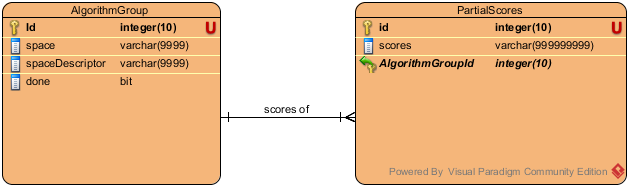
\includegraphics[width=0.9\textwidth]{data_diagram.png}
\caption{Model danych dla bazy relacyjnej}
\label{proj:diagram_data}
\end{figure}

Tabela \emph{AlgorithmGroup} stanowi reprezentację obliczeń związanych z pojedynczą grupą algorytmów. Atrybut space jest zserializowanym obiektem klasy \emph{SearchSpace}. Atrybut ten jest potrzebny, aby program przetwarzający informacje o grupach miał dostęp do szczegółów każdej z nich. Atrybut \emph{spaceDescriptor} to czytelny opis grupy algorytmów. Ostatni atrybut o nazwie \emph{done} przechowuje wartość 0 lub 1 i wskazuje czy obliczenia dla danej grupy zostały ukończone, czy nie. Kolumna \emph{id} to unikalny identyfikator wiersza.

Dla każdego wiersza w tabeli AlgorithmGroup istnieje przynajmniej jeden wiersz w tabeli PartialScores. Tabela ta przechowuje cząstkowe wyniki obliczeń pochodzące z pojedynczego programu wykonującego obliczenia. Zbiór wszystkich wierszy tabeli PartialScores $P_a$ odpowiadający konkretnemu wierszowi tabeli AlgorithmGroup $a$ zawiera wszystkie wyniki oceny klasyfikacji grupy algorytmów opisanej w $a$.

Kolumna \emph{id} tabeli \emph{PartialScores} to unikalny identyfikator wiersza. Pole \emph{scores} to zserializowana tablica trójek wartości - miary wrażliwości, precyzji i F1. \emph{AlgorithmGroupId} to klucz obcy tabeli.

\section{Program nadzorujący obliczenia}
\label{proj:supervisor}

Program nadzorujący obliczenia ma za zadanie pobrać od użytkownika opis grupy algorytmów do oceny, dokonać oceny oraz zapisać wyniki do bazy danych. Część ta skupia się na opisie algorytmów oraz klas użytych w programie nadzorującym.

\subsection{Interfejs użytkownika}

Nadzorca jest aplikacją konsolową. Szczegóły dotyczące uruchomienia obliczeń przekazywane są jako argumenty linii poleceń. Tabela \ref{proj:table_calculate_args} zwiera zwięzły opis argumentów programu. 

\begin{table}[h]
\begin{center}
\begin{tabular}{ | l | p{110mm} | }
\hline
\rowcolor{lightgray} Parametr & Opis \\\hline

-f \emph{metody} & Lista metod imputacji danych.\\\hline
-rc \emph{atrybuty} & Lista atrybutów przeznaczonych do usunięcia.\\\hline
-rs \emph{rozmiary} & Lista rozmiarów podzbiorów atrybutów przeznaczonych do usunięcia.\\\hline
-nc \emph{atrybuty} & Lista atrybutów przeznaczonych do przeskalowania.\\\hline
-ns \emph{rozmiary} & Lista rozmiarów podzbiorów atrybutów przeznaczonych do przeskalowania.\\\hline
-qc \emph{atrybuty} & Lista atrybutów, które mogą być użyte podczas grupowania.\\\hline
-qa \emph{algorytmy} & Lista algorytmów grupowania, których kombinacje mają być użyte.\\\hline
-qs \emph{liczności} & Lista liczności algorytmów grupowania, które mają być uruchomione jednocześnie na rozłącznych podzbiorach atrybutów.\\\hline
-qm \emph{liczba} & Maksymalna liczba atrybutów grupowanych jednocześnie przez pojedynczy algorytm grupowania.\\\hline
-qg \emph{granularność} & Granularność algorytmów grupowania.\\\hline
-cg \emph{granularność} & Granularność algorytmów klasyfikacji.\\\hline
-gs \emph{rozmiar} & Maksymalny rozmiar pojedynczego bloku algorytmów.\\\hline
-ws \emph{rozmiar} & Maksymalny rozmiar puli zadań obserwowanych przez nadzorcę.\\\hline
-r & Nadpisz istniejące wyniki dla grupy algorytmów.\\\hline
-s & Utwórz nowe ziarno pseudolosowe.\\\hline

\end{tabular}
\caption{Argumenty programu nadzorującego obliczenia.}
\label{proj:table_calculate_args}
\end{center}
\end{table}

Jak można zauważyć, argumenty programu umożliwiają sprecyzowanie grupy algorytmów tak, jak jest to opisane w rozdziale poświęconym założeniom i wymaganiom systemu. Interfejs pozwala tworzyć nowe ziarna pseudolosowe używane do podziału zbioru danych podczas walidacji krzyżowej. Nadzorca zapisuje informacje o wynikach oceny w bazie danych i, w razie ponownego uruchomienia dla tej samej grupy algorytmów, nie wykonuje żadnej akcji. Argument \emph{-r} pozwala ,,zresetować'' stan wiedzy o wynikach i uruchomić obliczenia jeszcze raz.

Argumenty programu parsowane są przez klasę o nazwie \emph{Parser}. Zadaniem klasy jest przyjęcie ciągów znaków (argumentów), przeanalizowanie go i wyprodukowanie struktury danych typu \emph{CmdArguments} zawierającej pola odpowiadające poszczególnym argumentom.

\subsection{Zarządzenie obliczeniami równoległymi}

Po otrzymaniu parametrów zgromadzonych w obiekcie klasy \emph{CmdArguments}, aplikacja może rozpocząć właściwe działanie. W głównym wątku aplikacji obiekt $app$ klasy \emph{CalculateApplication} odczytuje z bazy danych informacje o tym czy obliczenia powinny być rozpoczęte, czy wznowione od pewnego momentu. Następnie tworzony jest obiekt klasy \emph{TimeLeftEstimator} służący do estymacji czasu trwania reszty obliczeń. Kolejnym korkiem jest utworzenie obiektu $procedure$ klasy \emph{EvaluationProcedure}, który zawiera w sobie całą logikę zarządzania obliczeniami rozproszonymi. Obiekt ten powołuje do życia nowy wątek w którym wysyła do programów-robotników zlecenia oceny algorytmów. Obiekt $app$ na bieżąco monitoruje postęp działania obiektu $procedure$ i wyświetla go na ekranie razem z estymatą zakończenia obliczeń. Ilekroć obiekt $procedure$ odbierze oceny pewnych algorytmów, wywołuje funkcję ,,callback'' obiektu $app$, która zapisuje oceny w  bazie danych. Program kończy swe działanie gdy obliczenia się zakończą lub gdy użytkownik wciśnie kombinację klawiszy \emph{Ctrl+C}. 

\subsubsection{Klasa TimeLeftEstimator}

Klasa \emph{TimeLeftEstimator} służy do przewidzenia, kiedy obliczenia się zakończą, na podstawie tempa postęp tych obliczeń.

\begin{figure}[h]
\centering
\begin{tikzpicture} 
\umlclass{TimeLeftEstimator}{
}{
  + getElapsed(): TimeDelta\\
  + start()\\
  + update(progress: Float)\\
}
\end{tikzpicture}
\caption{Diagram UML klasy \emph{TimeLeftEstimator}}
\label{proj:diagram_time_left_est}
\end{figure}

Metoda \emph{start()} rozpoczyna pomiar czasu przez estymator. Metoda \emph{update()} przyjmuje jeden parametr - postęp obliczeń wyrażony jako liczba z przedziału [0, 1]. Metoda ta uaktualnia wewnętrzny stan obiektu. Metoda o nazwie \emph{getElapsed} zwraca domniemany czas potrzebny na zakończenie obliczeń.

\subsubsection{Klasa CalculateApplication}

Podstawę prezentacji i komunikacji z użytkownikiem stanowi klasa \emph{CalculateApplication}. Konstruktor klasy pobiera trzy parametry. Pierwszym z nich jest obiekt klasy \emph{CmdArguments} reprezentujący argumenty linii poleceń. Następnym parametrem jest URL serwera bazy danych. Ostatnim parametrem jest ścieżka do pliku z zapisanym ziarnem pseudolosowym.

Metoda \emph{resetSpace()} usuwa z bazy danych wpis o obliczeniach dotyczących aktualnej grupy algorytmów wybranej przez użytkownika. 

Ziarno pseudolosowe może być wygenerowane ponownie i zapisane do pliku dzięki metodzie \emph{recreateRandomState()}.

Ilekroć nadzorca odbiera nowe wyniki obliczeń, następuje potrzeba zapisania ich do bazy danych. Metoda \emph{updateResults()} jest funkcją typu callback obiektu klasy \emph{CalculateApplication} i jest wywoływana z osobnego wątku przez obiekt klasy \emph{EvaluationProcedure} ilekroć pojawią się nowe oceny algorytmów.

Metoda \emph{run()} odpowiada za uruchomienie obliczeń w programie. Całość prezentuje rysunek \ref{proj:diagram_calculate_application}.

\begin{figure}[h]
\centering
\begin{tikzpicture} 
\umlclass{CalculateApplication}{
}{
  + CalculateApplication(args: CmdArguments, url: String,\\ randomFilename: String)\\
  + recreateRandomState()\\
  + resetSpace()\\
  + run()\\
  + updateResults(scores: Array[Float])\\
}
\end{tikzpicture}
\caption{Diagram UML klasy \emph{CalculateApplication}}
\label{proj:diagram_calculate_application}
\end{figure}

\subsubsection{Klasa EvaluationProcedure}

Zarządzanie przeprowadzaniem obliczeń powinno przebiegać w następujący sposób. Nadzorca generuje wszystkie algorytmy wchodzące w skład zdefiniowanej przez użytkownika grupy algorytmów. Następnie tworzona jest pusta pula zadań, które są aktualnie wykonywanie przez robotników. Nadzorca przydziela algorytmy do zadań, które następnie umieszcza w puli. Dodanie zadania do puli jest jednoznaczne z wysłaniem zadania do systemu kolejkowego i rozpoczęciem obserwowania jego postępów. Pula zadań ma ustalony maksymalny rozmiar, np. 100 zadań monitorowanych jednocześnie. Gdy któreś zadanie zostanie ukończone, nadzorca odbiera wyniki z systemu kolejkowego, umieszcza je w bazie danych i dodaje do puli nowe zadanie. Nadzorca kończy pracę gdy zadania się wyczerpią i gdy wszystkie zadania zostaną ukończone.

Jak zostało to powiedziane w części \ref{req:research_scheme}, prowadząc obliczenia na wielu maszynach, należy mieć na uwadze wpływ opóźnień w sieci na wydajność systemu. Proces nadzorujący obliczenia powinien zatem wysyłać bloki deskryptorów, a nie pojedyncze deskryptory. Przesyłanie informacji o algorytmach do oceny w dużych grupach minimalizuje narzut związany z komunikacją sieciową. 

Klasa \emph{EvaluationProcedure} jest odpowiedzialna za zarządzanie wykonywaniem obliczeń w nadzorcy. Konstruktor klasy przyjmuje pięć parametrów. Pierwszym z nich jest ścieżka do pliku z danymi. Drugi parametr to to obiekt klasy \emph{SearchSpace}. Kolejny parametr to obiekt reprezentujący ziarno pseudolosowe. Czwartym parametrem konstruktora jest rozmiar bloku wysyłanych deskryptorów. Ostatnim parametrem jest rozmiar puli zadań.

\begin{figure}[h]
\centering
\begin{tikzpicture} 
\umlclass{EvaluationProcedure}{
}{
  + EvaluationProcedure(filepath: String, space: SearchSpace,\\ random: RandomState, blockSize: Int, poolSize: Int)\\
  + getProgress(): Float\\
  + isDone(): Boolean\\
  + start()\\
  + stop()\\
}
\end{tikzpicture}
\caption{Diagram UML klasy \emph{EvaluationProcedure}}
\label{proj:diagram_evaluation_procedure}
\end{figure}

Zarządzanie obliczeniami rozpoczyna się po wywołaniu metody \emph{start()}. Metoda \emph{stop()} wstrzymuje pracę. Aby uzyskać informacje o całkowitym postępie obliczeń należy użyć metody \emph{getProgress()}. Zwraca ona liczbę z przedziału [0, 1] odpowiadającą zaawansowaniu wykonywanych obliczeń. Metoda \emph{isDone()} pozwala stwierdzić czy obliczenia zostały ukończone.

\subsection{Warstwa dostępu do danych}

Dostęp do danych w bazie zapewnia obiekt klasy DataStore. Metody klasy umożliwiają dodawanie informacji o analizowanej grupie algorytmów, dodawanie wyników cząstkowych do badanej grupy, usuwanie grupy oraz przeglądanie grup algorytmów zapisanych w bazie. Klasę DataStore przedstawia rysunek \ref{proj:diagram_data_store}.

\begin{figure}[h]
\centering
\begin{tikzpicture} 
\umlclass{DataStore}{
}{
  + DataStore(url: String)\\
  + addScores(space: SearchSpace, scores: Array[Float])\\
  + delete(space: SearchSpace)\\
  + getScores(space: SearchSpace): Array[Float]\\
  + getSpaces(): Array[SearchSpace]\\
  + markDone(space: SearchSpace)\\
}
\end{tikzpicture}
\caption{Diagram UML klasy \emph{DataStore}}
\label{proj:diagram_data_store}
\end{figure}

Konstruktor klasy \emph{DataStore} przyjmuje jeden argument - adres URL serwera bazy danych.

Dodawanie wyników do bazy realizowane jest poprzez wołania metody \emph{addScores()}. Pierwszym parametrem metody jest obiekt klasy \emph{SearchSpace} opisujący grupę algorytmów, do której należy dodać wyniki. Drugim parametrem metody jest tablica wartości ocen jakości klasyfikacji. Metoda \emph{addScores()} dodaje wyniki do istniejącego wiersza w tabeli \emph{AlgorithmGroup}. Jeżeli wiersz w tabeli nie istnieje, zostanie on utworzony przez metodę.

Zadaniem metody o nazwie delete jest usunięcie z bazy informacji o obliczeniach dotyczących wybranej grupy algorytmów. Parametrem metody jest obiekt klasy \emph{SearchSpace} reprezentujący tę grupę.

Metoda \emph{getScores()} zwraca tablicę wyników ocen wybranej grupy algorytmów. Parametrem metody jest obiekt klasy \emph{SearchSpace}.

W celu uzyskania informacji o wszystkich grupach algorytmów, dla których obliczenia były prowadzone, należy wywołać metodę \emph{getSpaces()}. Zwróci ona tablicę obiektów klasy \emph{SearchSpace}.

Ostatnią metodą publiczną klasy \emph{DataStore} jest \emph{markDone()}. Metoda to oznacza grupę algorytmów jako taką, dla której wszystkie obliczenia zostały ukończone.

\section{Program liczący}

Zadaniem programu liczącego jest odbieranie zadań z systemu kolejkowego, wykonywanie niezbędnych obliczeń i zwracanie wyników do systemu kolejkowego.

Odbieranie zadań jest zapewnione przez biblioteki programistyczne dostarczone przez twórców systemu kolejkowego. Wykonywanie obliczeń polega na wytworzeniu zbioru metryk klasyfikacji dla każdego algorytmu zawartego w bloku dostarczonym razem z zadaniem. Metryki są łączone w jeden zbiór i wysyłane z powrotem do systemu kolejkowego jako rezultat pojedynczego zadania.

Program liczący używa biblioteki \emph{mltool} w celu przeprowadzenia obliczeń oraz bibliotek związanych z systemem kolejkowym aby odebrać zadanie i wysłać wyniki.

\section{Prezentowanie wyników obliczeń}

Celem obliczania metryk jakości klasyfikacji dla grup algorytmów jest ich późniejsza analiza. Badanie polega na przyglądaniu się cechom wyników wewnątrz grup (np. wartość średnia, odchylenie standardowe, kształt rozkładu) oraz na porównaniu wyników między grupami. Do realizacji tych zadań służą programy \emph{browse} i \emph{compare}.

\subsection{Program browse}

Program \emph{browse} służy do przeglądu otrzymanych wyników jakości klasyfikacji grup algorytmów. Program umożliwia przegląd wyników wybranych grupa algorytmów lub wszystkich z nich.

\subsubsection{Interfejs użytkownika}

Użytkownik ma wpływ na działanie programu poprzez konsolowy interfejs. Argumenty programu \emph{browse} prezentuje tabela \ref{proj:table_browse_args}.

\begin{table}[h]
\begin{center}
\begin{tabular}{ | l | p{110mm} | }
\hline
\rowcolor{lightgray} Parametr & Opis \\\hline

-a \emph{akcja} & Wybór metody przeglądania. Możliwe wartości akcji to \emph{list} i \emph{plot}.\\\hline
-ids \emph{identyfikatory} & Lista identyfikatorów grup algorytmów, o których informacje należy wyświetlić.\\\hline
-m \emph{metryka} & Rodzaj metryki, którą należy wyświetlić.\\\hline

\end{tabular}
\caption{Argumenty programu \emph{browse}.}
\label{proj:table_browse_args}
\end{center}
\end{table}

Wyświetlanie informacji o wynikach grup działa na dwa sposoby. Tryb pierwszy wyświetla szczegółową listę grup algorytmów oraz informacje o wynikach tj. średnie wartości metryk, liczba algorytmów w grupie. Tryb drugi wyświetla histogramy wybranej metryki dla ustalonych grup algorytmów. Do przełączania trybów pracy służy argument \emph{-a}.

Program \emph{browse} pozwala wybrać grupy algorytmów, które mają być pokazane na ekranie. Do wyboru służy opcja \emph{-ids.} Jeżeli opcja ta nie jest sprecyzowana, zostaną wyświetlone wszystkie grupy.

Podczas wyświetlania histogramów wybranych metryk należy wybrać rodzaj metryki. Służy do tego argument \emph{-m}. Jeżeli argument ten nie jest jawnie zdefiniowany, domyślnym rodzajem oceny jest metryka F1.

\subsubsection{Struktura programu}

Program \emph{browse} posiada klasę o nazwie \emph{BrowseCmdParser} odpowiedzialną za parsowanie argumentów linii poleceń. Metoda \emph{parse()} klasy \emph{BrowseCmdParser} zwraca strukturę zawierającą pola odpowiadające argumentom linii poleceń. 

Aplikacja używa biblioteki \emph{mltool} w celu przetwarzania wyników poszczególnych grup (np. liczenie histogramu) oraz bibliotek umożliwiających komunikację z bazą danych.

\subsection{Program compare}

Porównywanie wyników grup algorytmów między sobą jest realizowane przez program o nazwie \emph{compare}. Efektem działania programu jest ranking grup zgodny z założeniami opisanymi w części \ref{req:research_scheme}.

\subsubsection{Interfejs programu}

Program \emph{compare} jest aplikacją konsolową. Argumenty linii poleceń programu pokazane są w tabeli \ref{proj:table_compare_args}.

\begin{table}[h]
\begin{center}
\begin{tabular}{ | l | p{110mm} | }
\hline
\rowcolor{lightgray} Parametr & Opis \\\hline

-p \emph{poziom} & Poziom istotności (od 0 do 1) dla testu Manna-Whitneya-Wilcoxona.\\\hline
-o \emph{metryka} & Metryka wg której tworzony jest ranking.\\\hline
-c \emph{liczba} & Liczba najlepszych pozycji w rankingu do wyświetlenia.\\\hline

\end{tabular}
\caption{Argumenty programu \emph{compare}.}
\label{proj:table_compare_args}
\end{center}
\end{table}

\subsubsection{Struktura aplikacji}

Klasa \emph{CompareCmdParser} pozwala na parsowanie argumentów linii poleceń i otrzymanie struktury zawierającej odpowiadające im pola. 

Program \emph{compare} używa biblioteki \emph{mltool}, bibliotek umożliwiających komunikację z bazą danych oraz bibliotek matematycznych posiadających implementację testu Manna-Whitneya-Wilcoxona.

\section{Testy}

Biblioteka obliczeniowa \emph{mltool} stanowi fundament całej aplikacji. Wyniki działania biblioteki decydować będą o rezultatach badań, jakie przeprowadzać będzie użytkownik. Z tego powodu niezmiernie istotne jest upewnienie się, że biblioteka obliczeniowa działa poprawnie. 

W celu sprawdzenia tego istotnego warunku, poprawność działania klas w bibliotece będzie sprawdzana przy pomocy testów jednostkowych. Dzięki modularnej strukturze biblioteki opisanej w punkcie~\ref{proj:sec_structure}, możliwe jest oddzielne testowanie poszczególnych klas biblioteki. Weryfikacja poprawności działania poszczególnych fragmentów biblioteki umożliwi wyeliminowanie większości możliwych błędów.

Tabela \ref{proj:table_mltool_input} prezentuje opis testów jednostkowych badających poprawność działania części biblioteki odpowiedzialnej za odczyt i przetwarzanie wstępne danych. Testy klas-modeli pokazuje tabela \ref{proj:table_mltool_models}. W tabeli \ref{proj:table_mltool_descriptors} zaprezentowane są testy badające poprawność deskryptorów. Testy klas generujących algorytmy wewnątrz grup algorytmów opisane są w tabeli \ref{proj:table_mltool_spaces}.

\begin{table}[h]
\begin{center}
\begin{tabular}{ | l | p{110mm} | }
\hline
\rowcolor{lightgray} Nazwa klasy & Opis testów \\\hline

XlsFile & Badanie poprawności odczytu danych prawidłowych oraz badanie reakcji na próbę odczytu danych nieprawidłowych. \\\hline
Sample & Badanie poprawności odczytu danych prawidłowych oraz badanie reakcji na próbę odczytu danych nieprawidłowych. Sprawdzenie poprawnego działania metod \emph{getNormalizer}, \emph{removeColumns}, \emph{impute}, \emph{normalize}, \emph{mergeColumns}.\\\hline

\end{tabular}
\caption{Opis testów klas biblioteki \emph{mltool} związanych z odczytem i reprezentacją danych.}
\label{proj:table_mltool_input}
\end{center}
\end{table}

\begin{table}[h]
\begin{center}
\begin{tabular}{ | l | p{110mm} | }
\hline
\rowcolor{lightgray} Nazwa klasy & Opis testów \\\hline

Imputer & Sprawdzenie poprawnego działania metod \emph{fit} i \emph{transform}.\\\hline
Normalizer & Sprawdzenie poprawnego działania metod \emph{fit} i \emph{transform}.\\\hline
Clusterer & Sprawdzenie poprawnego działania metod \emph{fit} i \emph{transform}.\\\hline
NaiveBayesClassifier & Badanie poprawnego działania metody \emph{fit}. Sprawdzenie czy predykcja metodą \emph{predict()} spełnia podstawowe założenia dotyczące przewidywania kategorii.\\\hline
DecisionTreeClassifier & Sprawdzenie poprawnego działania metody \emph{fit}. Sprawdzenie czy predykcja metodą \emph{predict()} spełnia podstawowe założenia dotyczące przewidywania kategorii.\\\hline
SVMClassifier & Badanie poprawnego działania metody \emph{fit}. Sprawdzenie czy predykcja metodą \emph{predict()} spełnia podstawowe założenia dotyczące przewidywania kategorii.\\\hline
RandomForestClassifier & Sprawdzenie poprawnego działania metody \emph{fit}. Sprawdzenie czy predykcja metodą \emph{predict()} spełnia podstawowe założenia dotyczące przewidywania kategorii.\\\hline

\end{tabular}
\caption{Opis testów klas-modeli biblioteki \emph{mltool}.}
\label{proj:table_mltool_models}
\end{center}
\end{table}

\begin{table}[h]
\begin{center}
\begin{tabular}{ | l | p{110mm} | }
\hline
\rowcolor{lightgray} Nazwa klasy & Opis testów \\\hline

PreprocessingDescriptor & Wywoływanie metody \emph{validate} dla poprawnych i niepoprawnych ustawień deskryptora. Sprawdzanie czy dla danych nieprawidłowych metoda \emph{validate} rzuca wyjątkiem DescriptorException. Badanie czy metody \emph{cluster} i \emph{impute} zwracają właściwe wyniki.\\\hline
GroupingDescriptor & Uruchamianie metody \emph{validate} dla poprawnych i niepoprawnych ustawień deskryptora. Sprawdzanie czy dla danych nieprawidłowych metoda \emph{validate} rzuca wyjątkiem DescriptorException. Sprawdzanie czy metoda \emph{createAlgorithm} zwraca poprawny wynik.\\\hline
ClassificationDescriptor & Sprawdzenie czy metoda \emph{createClassifier} działa poprawnie. Wywoływanie metody \emph{validate} dla poprawnych i niepoprawnych ustawień deskryptora. Sprawdzanie czy dla danych nieprawidłowych metoda \emph{validate} rzuca wyjątkiem DescriptorException.\\\hline

\end{tabular}
\caption{Opis testów deskryptorów w bibliotece \emph{mltool}.}
\label{proj:table_mltool_descriptors}
\end{center}
\end{table}

\begin{table}[h]
\begin{center}
\begin{tabular}{ | l | p{110mm} | }
\hline
\rowcolor{lightgray} Nazwa klasy & Opis testów \\\hline

ImputeSpace & Sprawdzenie czy metoda \emph{generate} wytwarza wyniki zgodne z parametrami obiektu.\\\hline
RemoveSpace & Wywołanie metody \emph{generate} dla obiektu klasy \emph{RemoveSpace} i sprawdzenie czy zwrócone obiekty klasy \emph{PreprocessingDescriptor} są zgodne z założeniami.\\\hline
ScaleSpace & Badanie czy efektem wywołania metody \emph{RemoveSpace} jest tablica prawidłowych obiektów klasy \emph{PreprocessingDescriptor}. Sprawdzenie tego warunku dla wariantu z usuwaniem atrybutów i bez usuwania. \\\hline
GroupingSpace & Sprawdzenie czy metoda \emph{generate} zwraca kolekcję obiektów zgodną z ustawieniami obiektu \emph{GroupingSpace}.\\\hline
ClassificationSpace & Wywołanie metody \emph{generate} i zbadanie czy wygenerowanie deskryptory klasyfikacji są prawidłowe.\\\hline
SearchSpace & Sprawdzenie czy metoda \emph{generate} generuje wszystkie warianty par deskryptorów przetwarzania wstępnego i klasyfikacji.\\\hline

\end{tabular}
\caption{Opis testów klas upraszczających generowanie algorytmów w bibliotece \emph{mltool}.}
\label{proj:table_mltool_spaces}
\end{center}
\end{table}

\end{document}
